\documentclass[11pt,a4paper]{extarticle}
\usepackage[latin1]{inputenc}
\usepackage{amsmath}
\usepackage{microtype}
\usepackage[none]{hyphenat}
\usepackage{verbatim}
\usepackage{amsfonts}
\usepackage{amssymb}
\usepackage{enumitem}
\renewcommand{\familydefault}{\sfdefault}
\usepackage{mathpazo}
\renewcommand{\rmdefault}{put}
\usepackage{enumitem}
\usepackage[dvipsnames,svgnames]{xcolor}
\usepackage{tkz-euclide}
\usetkzobj{all}
\usepackage{graphicx}
\usepackage{tikz} 	
\usepackage{adjustbox}
\usepackage{multicol}
\usepackage{lipsum}
\usepackage[left=0.7cm,right=1cm,top=1cm,bottom=1.5cm]{geometry}
\usepackage{cancel} \usepackage{xcolor}
\usepackage{tcolorbox}
\usetikzlibrary{decorations.pathmorphing,patterns}
\usetikzlibrary{decorations.pathreplacing,calc}
 \newcommand\coret[2][red]{\renewcommand\CancelColor{\color{#1}}\cancel{#2}}
\SetLabelAlign{Center}{\hfil\makebox[1.0em]{#1}\hfil}

%%_------= solusi


% Set this =0 to hide, =1 to show

% Set this =0 to hide, =1 to show
\newtcolorbox{mybox}[1][] { colframe = blue!10, colback = blue!3,boxsep=0pt,left=0.2em, coltitle = blue!20!black, title = \textbf{jawab}, #1, } 

%---------- kunci (jika 1 ) muncul
\def\tampilkunci{1}
\newcommand{\hide}[1]{\ifnum\tampilkunci=1
%
\begin{mybox}
 #1
\end{mybox}
%
\vspace{\baselineskip}\fi}



\newcommand*\cicled[1]{\tikz[baseline=(char.base)]{\node[white, shape=circle, fill=red!80,draw,inner sep=0.5pt](char){#1};}}

\newcommand*\kunci[1]{\ifnum\tampilkunci=1
%
\tikz[baseline=(char.base)]{\node[red, shape=circle,draw,inner sep=0.5pt,xshift=2pt](char){#1};}\stepcounter{enumii}
\fi\ifnum\tampilkunci=0
%
\hspace{3pt}#1\stepcounter{enumii}
%
\fi}

\newcommand*\silang[1]{\tikz[baseline=(char.base)]{
\draw[red,thick](-0.2,-0.20)--(0.2,0.2);
\draw[red,thick](-0.2,0.20)--(0.2,-0.2);
\node[black](char){#1};
}}

\newcommand*\centang[1]{\tikz[baseline=(char.base)]{
\draw[red, very thick](-0.2,0.1)--(-0.1,0)--(0.2,0.3);
\node(char){#1};
}}

\newcommand*\merah[1]{
\textcolor{red}{#1}}
\newcommand*\pilgan[1]{
\begin{enumerate}[label=\Alph*., itemsep=0pt,topsep=0pt,leftmargin=*,align=Center] #1 
\end{enumerate}}
\newcommand*\pernyataan[1]{
\begin{enumerate}[label=(\arabic*), itemsep=0pt,topsep=0pt,leftmargin=*] #1 
\end{enumerate}}

\newcommand*\daftar[1]{
\begin{itemize}[label=$\bullet$, itemsep=0pt,topsep=0pt,leftmargin=*] #1 
\end{itemize}}


\newcommand{\pilgani}[1]{                            \vspace{-0.3cm}\begin{multicols}{2}
 \begin{enumerate}[label=\Alph*., itemsep=0pt,topsep=0pt,leftmargin=*,align=Center]#1                     \end{enumerate}
 \phantom{ini cuma sapi, wedus, dan ayam}
 \end{multicols}}


\begin{document}


 \textbf{Ringkasan dan Latihan Momentum} \phantom{ini nama siswa yang aaamengerjakan soal kuis ini }  

\begin{multicols*}{2}
\textbf{Momentum}

Momentum adalah tingkat kesulitan kesulitan untuk menghentikan benda. Faktor yang mempengaruhi adalah $m$ (massa) dan $v$ (kecepatan)

$$ p = m v \text{  (Ns)}$$

Momentum bersifat vektor, sehingga memperhatikan arah ( + / - ) dan sudut vektor 


\begin{enumerate}
\item Sebuah benda kecepatannya 20 m/s, dengan massa 1000 kg. Maka momentum benda tersebut adalah 
\pilgani{
        \item 10.000 Ns
        \item 20.000 Ns
        \item 30.000 Ns
        \item 40.000 Ns
        \item 50.000 Ns
        }
\item Bola A bermassa 2 kg bergerak ke sumbu-$x$ dengan kecepatan 20 m/s dan bola B dengan massa 1 kg bergerak ke sumbu-$y$ 30 m/s. Jumlah momentum kedua benda adalah . . .
\pilgani{
        \item 70 Ns
        \item 10 Ns
        \item -10 Ns
        \item 50 Ns
        \item 20 Ns
        }

\item Balok A bermassa 1 kg bergerak ke sumbu-$x$ dengan kecepatan 10 m/s, balok B bermassa 3 kg bergerak dengan kecepatan sama ke arah 30$^o$ dari sumbu-$y$. Total momentum kedua benda tersebut adalah . . .
\pilgani{
        \item $10\sqrt{10+1,5\sqrt{3}}$
        \item $10\sqrt{13}$
        \item $10$
        \item $40$
        \item --20
        }

\textbf{Kekekalan Momentum}

\begin{align*}
\Sigma p &= \Sigma p'\\
m_1.v_1 + m_2.v_2 &= m_1.v_1' +m_2v_2'\\
\end{align*}

\item Sebuah benda bergerak dengan kecepatan berlawanan. Kecepatan A adalah 6 m/s, dan kecepatan B adalah $v$. Jika setelah bertumbukan, benda A dan B berbalik arah dengan kecepatan 4 m/s dan 2 m/s maka kecepatan awal B adalah . . . 
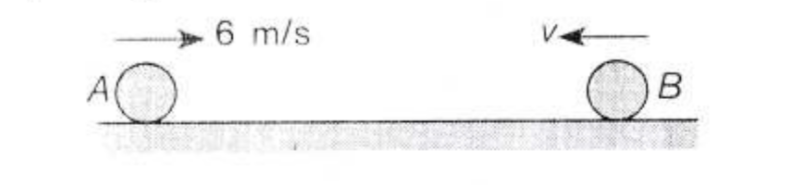
\includegraphics[width=8cm]{pic/mom1}
\pilgani{
        \item 6 m/s
        \item 3 m/s
        \item 1,6 m/s
        \item 1,2 m/s
        \item 0,4 m/s
        }

\vspace{2cm}

\textbf{Jenis tumbukan, koefisien restitusi $e$}
        \begin{enumerate}
\item Lenting sempurna
     \daftar{
        \item $e =1 $
        \item $\Sigma p = \Sigma p' $
        \item Energi kinetik kekal $EK=EK'$
        }

 \item Lenting Sebagian
        \daftar{
        \item $0<e<1$
        \item $\Sigma p = \Sigma p'$
        \item $EK> EK'$ artinya ada energi kinetik yang hilang, menjadi energi lain (misal: bunyi, panas, perubahan bentuk \textit{defomasi}}

 \item Tidak lenting sama sekali
        \daftar{
        \item $e=0$
        \item $\Sigma p = \Sigma p'$
        \item setelah bertumbukan kedua benda menjadi satu, sehingga 
        \item $m_Av_A + m_Bv_B = (m_A + m_B)v'$
        }
        \end{enumerate}


\end{enumerate}



\end{multicols*}\end{document}






